% Options for packages loaded elsewhere
% Options for packages loaded elsewhere
\PassOptionsToPackage{unicode}{hyperref}
\PassOptionsToPackage{hyphens}{url}
%
\documentclass[
  10pt,
  ignorenonframetext,
  aspectratio=169,
  russian,
]{beamer}
\newif\ifbibliography
\usepackage{pgfpages}
\setbeamertemplate{caption}[numbered]
\setbeamertemplate{caption label separator}{: }
\setbeamercolor{caption name}{fg=normal text.fg}
\beamertemplatenavigationsymbolshorizontal
% remove section numbering
\setbeamertemplate{part page}{
  \centering
  \begin{beamercolorbox}[sep=16pt,center]{part title}
    \usebeamerfont{part title}\insertpart\par
  \end{beamercolorbox}
}
\setbeamertemplate{section page}{
  \centering
  \begin{beamercolorbox}[sep=12pt,center]{section title}
    \usebeamerfont{section title}\insertsection\par
  \end{beamercolorbox}
}
\setbeamertemplate{subsection page}{
  \centering
  \begin{beamercolorbox}[sep=8pt,center]{subsection title}
    \usebeamerfont{subsection title}\insertsubsection\par
  \end{beamercolorbox}
}
% Prevent slide breaks in the middle of a paragraph
\widowpenalties 1 10000
\raggedbottom
\AtBeginPart{
  \frame{\partpage}
}
\AtBeginSection{
  \ifbibliography
  \else
    \frame{\sectionpage}
  \fi
}
\AtBeginSubsection{
  \frame{\subsectionpage}
}
\usepackage{iftex}
\ifPDFTeX
  \usepackage[T1]{fontenc}
  \usepackage[utf8]{inputenc}
  \usepackage{textcomp} % provide euro and other symbols
\else % if luatex or xetex
  \usepackage{unicode-math} % this also loads fontspec
  \defaultfontfeatures{Scale=MatchLowercase}
  \defaultfontfeatures[\rmfamily]{Ligatures=TeX,Scale=1}
\fi
\usepackage{lmodern}

\usetheme[]{metropolis}
\usefonttheme{serif} % use mainfont rather than sansfont for slide text
\ifPDFTeX\else
  % xetex/luatex font selection
  \setmainfont[]{DejaVu Sans}
  \setsansfont[]{DejaVu Sans}
  \setmonofont[]{DejaVu Sans Mono}
\fi
% Use upquote if available, for straight quotes in verbatim environments
\IfFileExists{upquote.sty}{\usepackage{upquote}}{}
\IfFileExists{microtype.sty}{% use microtype if available
  \usepackage[]{microtype}
  \UseMicrotypeSet[protrusion]{basicmath} % disable protrusion for tt fonts
}{}


\usepackage{longtable,booktabs,array}
\newcounter{none} % for unnumbered tables
\usepackage{calc} % for calculating minipage widths
\usepackage{caption}
% Make caption package work with longtable
\makeatletter
\def\fnum@table{\tablename~\thetable}
\makeatother
\usepackage{graphicx}
\makeatletter
\newsavebox\pandoc@box
\newcommand*\pandocbounded[1]{% scales image to fit in text height/width
  \sbox\pandoc@box{#1}%
  \Gscale@div\@tempa{\textheight}{\dimexpr\ht\pandoc@box+\dp\pandoc@box\relax}%
  \Gscale@div\@tempb{\linewidth}{\wd\pandoc@box}%
  \ifdim\@tempb\p@<\@tempa\p@\let\@tempa\@tempb\fi% select the smaller of both
  \ifdim\@tempa\p@<\p@\scalebox{\@tempa}{\usebox\pandoc@box}%
  \else\usebox{\pandoc@box}%
  \fi%
}
% Set default figure placement to htbp
\def\fps@figure{htbp}
\makeatother



\ifLuaTeX
\usepackage[bidi=basic,shorthands=off,provide=*]{babel}
\else
\usepackage[bidi=default,shorthands=off,provide=*]{babel}
\fi
\ifPDFTeX
\else
\babelfont{rm}[]{DejaVu Sans}
\fi
\ifLuaTeX
  \usepackage{selnolig} % disable illegal ligatures
\fi


\setlength{\emergencystretch}{3em} % prevent overfull lines

\providecommand{\tightlist}{%
  \setlength{\itemsep}{0pt}\setlength{\parskip}{0pt}}



 

\usepackage[]{csquotes}

%%% Load theme
\IfFileExists{beamerthemegotham.sty}{
  %%%% Full TeXlive
  \usetheme{gotham}
  \gothamset{
    numbering=totalframenumber,
    parttocframe default=off,
    sectiontocframe default=off,
    subsectiontocframe default=off,
    tocframe template=gotham bullet,
    % progressbar position=frametitle,
    progressbar position=foot,
  }
  \renewcommand{\gothamInstituteLogoSquare}[1][4ex]{%
    
\includegraphics[height=##1]{_resources/image/logo_rudn-inverted.png}
  }
  % \renewcommand{\gothamtitlepagelogo}[1][4ex]{%
  %   
\includegraphics[height=##1]{_resources/image/logo_rudn.png}
  % }
}{%
  %%%% TinyTeX
  \usepackage{libertine}
  %%%% https://deic.uab.cat/~iblanes/beamer_gallery/
  \usetheme{Madrid}
}
\metroset{progressbar=frametitle,numbering=fraction}
\setbeamersize{text margin left=8mm,text margin right=8mm}
\makeatletter
\@ifpackageloaded{caption}{}{\usepackage{caption}}
\AtBeginDocument{%
\ifdefined\contentsname
  \renewcommand*\contentsname{Содержание}
\else
  \newcommand\contentsname{Содержание}
\fi
\ifdefined\listfigurename
  \renewcommand*\listfigurename{Список иллюстраций}
\else
  \newcommand\listfigurename{Список иллюстраций}
\fi
\ifdefined\listtablename
  \renewcommand*\listtablename{Список таблиц}
\else
  \newcommand\listtablename{Список таблиц}
\fi
\ifdefined\figurename
  \renewcommand*\figurename{Рисунок}
\else
  \newcommand\figurename{Рисунок}
\fi
\ifdefined\tablename
  \renewcommand*\tablename{Таблица}
\else
  \newcommand\tablename{Таблица}
\fi
}
\@ifpackageloaded{float}{}{\usepackage{float}}
\floatstyle{ruled}
\@ifundefined{c@chapter}{\newfloat{codelisting}{h}{lop}}{\newfloat{codelisting}{h}{lop}[chapter]}
\floatname{codelisting}{Список}
\newcommand*\listoflistings{\listof{codelisting}{Листинги}}
\makeatother
\makeatletter
\makeatother
\makeatletter
\@ifpackageloaded{caption}{}{\usepackage{caption}}
\@ifpackageloaded{subcaption}{}{\usepackage{subcaption}}
\makeatother

\usepackage{bookmark}
\IfFileExists{xurl.sty}{\usepackage{xurl}}{} % add URL line breaks if available
\urlstyle{same}
% fallback for those not using the hyperref driver hyperxmp:
\makeatletter
\@ifundefined{xmpquote}{\newcommand{\xmpquote}[1]{#1}}{}
\makeatother
\hypersetup{
  pdftitle={Лабораторная работа № 4},
  pdfauthor={Нечаева Кира Андреевна},
  pdflang={ru-RU},
  hidelinks,
  pdfcreator={LaTeX via pandoc}}


\title{\texorpdfstring{Лабораторная работа №
4}{Лабораторная работа № 4}}
\subtitle{\texorpdfstring{Агентная модель SIR}{Агентная модель SIR}}
\author{Нечаева Кира Андреевна}
\date{}
\institute{НКНбд-01-23}

\begin{document}
\frame{\titlepage}


\begin{frame}{Цель работы}
\protect\phantomsection\label{ux446ux435ux43bux44c-ux440ux430ux431ux43eux442ux44b}
\textbf{Цель:} реализовать модель SIR в агентном подходе и исследовать
влияние параметров на эпидемическую динамику.

В работе:

\begin{itemize}
\tightlist
\item
  каждый человек представлен отдельным агентом;
\item
  агенты распределены между городами;
\item
  учитываются миграция и случайное заражение;
\item
  исследованы заразность и гетерогенность;
\item
  добавлена карантинная мера;
\item
  выполнена оптимизация параметров.
\end{itemize}
\end{frame}

\begin{frame}[fragile]{Агентная модель SIR}
\protect\phantomsection\label{ux430ux433ux435ux43dux442ux43dux430ux44f-ux43cux43eux434ux435ux43bux44c-sir}
\begin{columns}[c]
\begin{column}{0.39\linewidth}
Каждый агент имеет состояние:

\begin{itemize}
\tightlist
\item
  \texttt{S} --- восприимчивый;
\item
  \texttt{I} --- инфицированный;
\item
  \texttt{R} --- выздоровевший.
\end{itemize}

Дополнительно хранится количество дней после заражения.

Города представлены вершинами графа, между которыми агенты могут
перемещаться.
\end{column}

\begin{column}{0.61\linewidth}
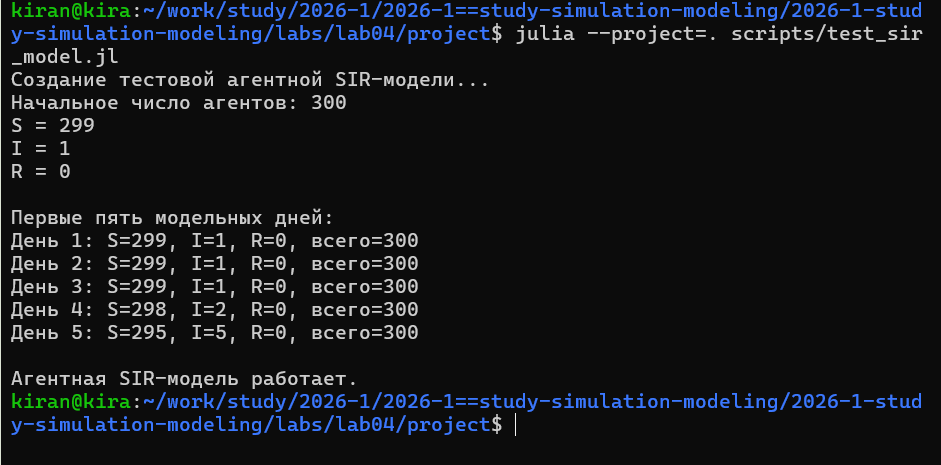
\includegraphics[width=1\linewidth,height=\textheight,keepaspectratio]{image/3.png}
\end{column}
\end{columns}
\end{frame}

\begin{frame}{Базовый эксперимент}
\protect\phantomsection\label{ux431ux430ux437ux43eux432ux44bux439-ux44dux43aux441ux43fux435ux440ux438ux43cux435ux43dux442}
\begin{columns}[c]
\begin{column}{0.31\linewidth}
В базовом сценарии:

\begin{itemize}
\tightlist
\item
  3 города;
\item
  по 1000 агентов;
\item
  один начальный инфицированный;
\item
  100 модельных дней.
\end{itemize}

Программа сама определяет:

\begin{itemize}
\tightlist
\item
  \(R_0\);
\item
  величину пика;
\item
  день пика;
\item
  число умерших.
\end{itemize}
\end{column}

\begin{column}{0.69\linewidth}
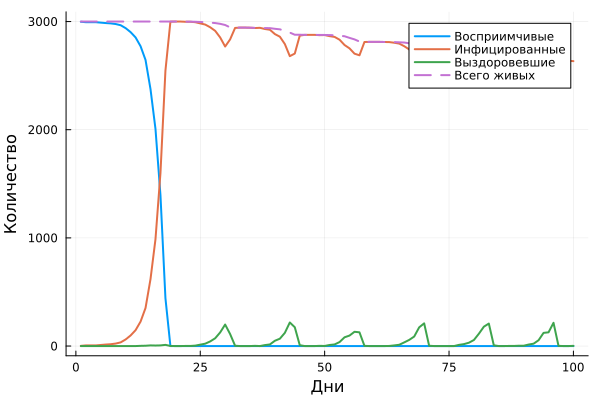
\includegraphics[width=1\linewidth,height=\textheight,keepaspectratio]{image/plots/sir_basic_dynamics.png}
\end{column}
\end{columns}
\end{frame}

\begin{frame}[fragile]{Влияние заразности}
\protect\phantomsection\label{ux432ux43bux438ux44fux43dux438ux435-ux437ux430ux440ux430ux437ux43dux43eux441ux442ux438}
\begin{columns}[c]
\begin{column}{0.3\linewidth}
Коэффициент \(\beta\) изменялся от 0.1 до 1.0.

Для каждого значения выполнено несколько прогонов с разными
\texttt{seed}.

После усреднения определяется порог возникновения эпидемии.
\end{column}

\begin{column}{0.7\linewidth}
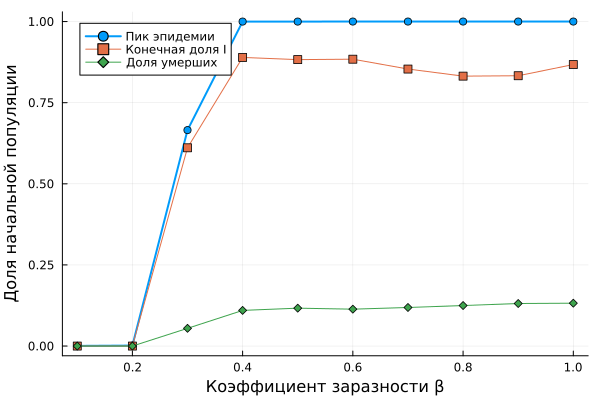
\includegraphics[width=1\linewidth,height=\textheight,keepaspectratio]{image/plots/beta_scan.png}
\end{column}
\end{columns}
\end{frame}

\begin{frame}{Гетерогенность городов}
\protect\phantomsection\label{ux433ux435ux442ux435ux440ux43eux433ux435ux43dux43dux43eux441ux442ux44c-ux433ux43eux440ux43eux434ux43eux432}
\begin{columns}[c]
\begin{column}{0.3\linewidth}
Для городов были заданы разные значения:

\[
\beta_1=0.2,\quad
\beta_2=0.5,\quad
\beta_3=0.8.
\]

Это позволяет отказаться от предположения об одинаковой эпидемической
ситуации во всех локациях.
\end{column}

\begin{column}{0.7\linewidth}
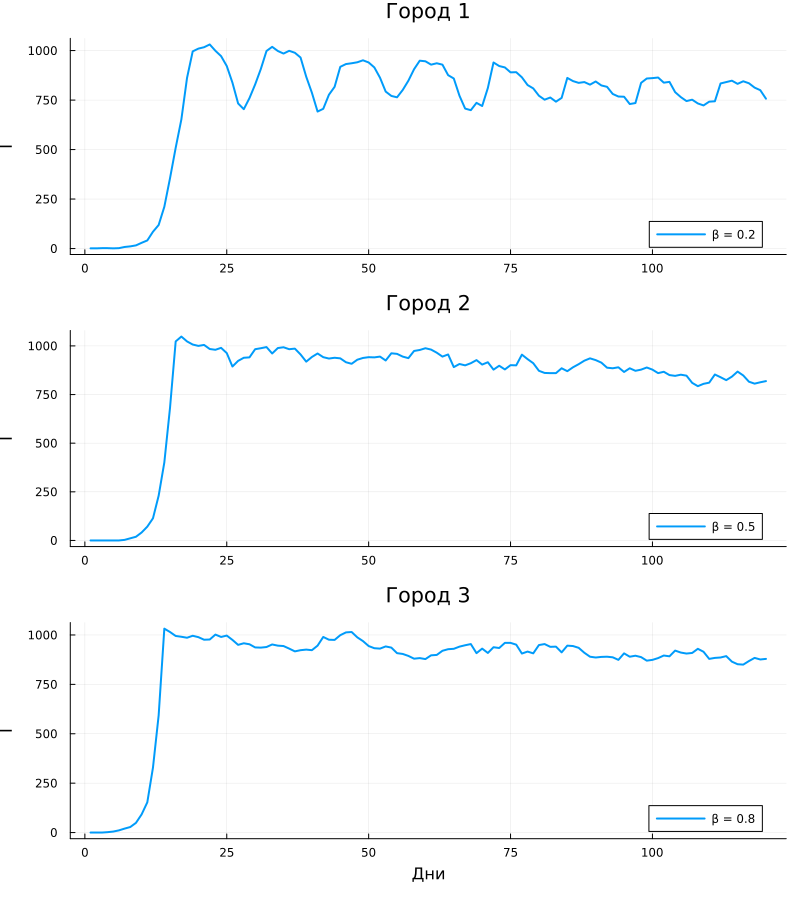
\includegraphics[width=0.88\linewidth,height=\textheight,keepaspectratio]{image/plots/heterogeneity_cities.png}
\end{column}
\end{columns}
\end{frame}

\begin{frame}{Влияние миграции}
\protect\phantomsection\label{ux432ux43bux438ux44fux43dux438ux435-ux43cux438ux433ux440ux430ux446ux438ux438}
\begin{columns}[c]
\begin{column}{0.31\linewidth}
Интенсивность перемещений между городами изменялась от 0 до 0.5.

Для каждого сценария рассчитывались:

\begin{itemize}
\tightlist
\item
  время до пика;
\item
  величина пика.
\end{itemize}

Матрица миграции создаётся программно для каждого эксперимента.
\end{column}

\begin{column}{0.69\linewidth}
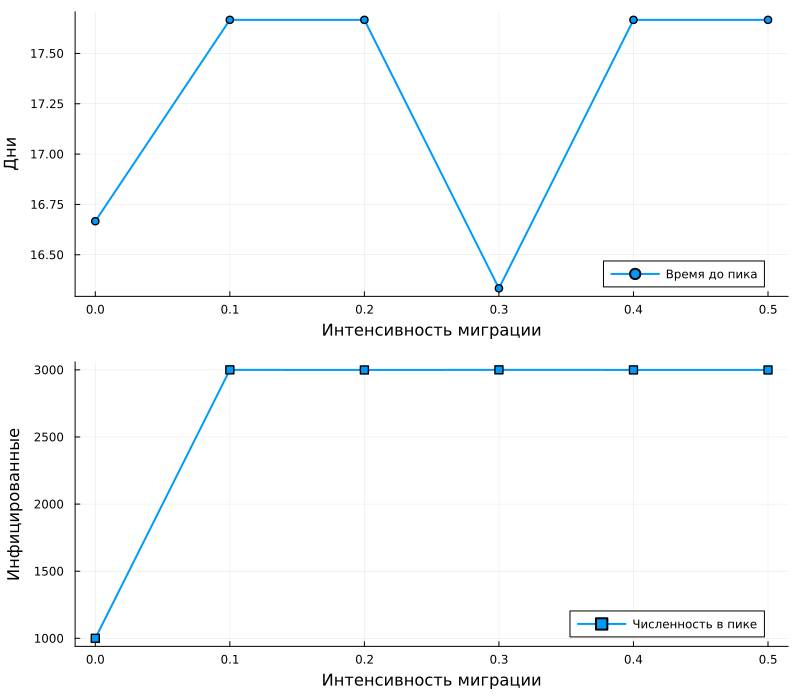
\includegraphics[width=0.95\linewidth,height=\textheight,keepaspectratio]{image/plots/migration_effect.png}
\end{column}
\end{columns}
\end{frame}

\begin{frame}[fragile]{Карантинная мера}
\protect\phantomsection\label{ux43aux430ux440ux430ux43dux442ux438ux43dux43dux430ux44f-ux43cux435ux440ux430}
\begin{columns}[c]
\begin{column}{0.31\linewidth}
При превышении порога заболеваемости город автоматически закрывается для
выезда.

Сравнивались два сценария:

\begin{itemize}
\tightlist
\item
  без ограничений;
\item
  с карантином.
\end{itemize}

Оба сценария запускаются с одинаковым \texttt{seed}.
\end{column}

\begin{column}{0.69\linewidth}
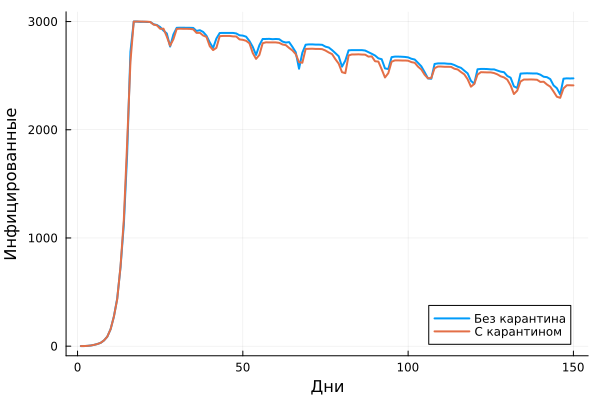
\includegraphics[width=1\linewidth,height=\textheight,keepaspectratio]{image/plots/quarantine_effect.png}
\end{column}
\end{columns}
\end{frame}

\begin{frame}{Оптимизация параметров}
\protect\phantomsection\label{ux43eux43fux442ux438ux43cux438ux437ux430ux446ux438ux44f-ux43fux430ux440ux430ux43cux435ux442ux440ux43eux432}
\begin{columns}[c]
\begin{column}{0.42\linewidth}
Автоматически подбирались:

\begin{itemize}
\tightlist
\item
  коэффициент заразности;
\item
  время выявления;
\item
  параметр смертности.
\end{itemize}

Цель --- уменьшить смертность при ограничении

\[
I_{\max} \leq 30\%.
\]

Превышение допустимого пика штрафуется целевой функцией.
\end{column}

\begin{column}{0.58\linewidth}
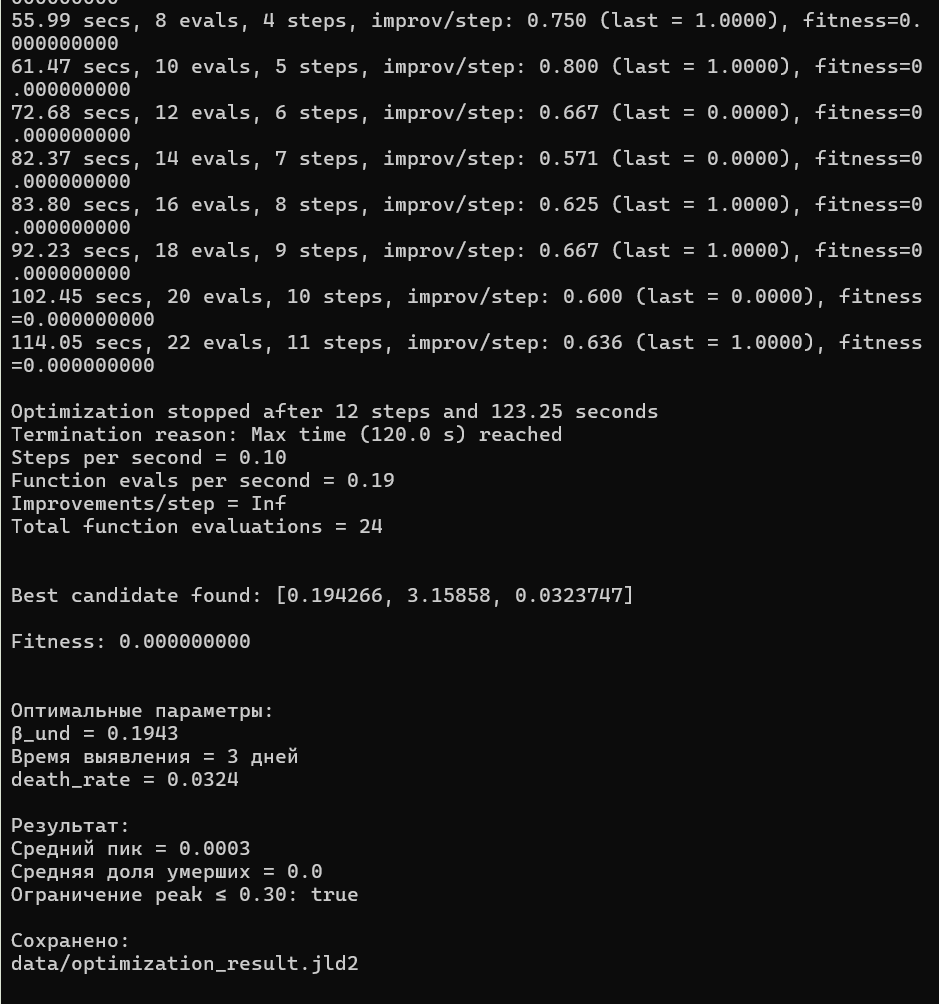
\includegraphics[width=1\linewidth,height=\textheight,keepaspectratio]{image/9.png}
\end{column}
\end{columns}
\end{frame}

\begin{frame}{Сводный анализ}
\protect\phantomsection\label{ux441ux432ux43eux434ux43dux44bux439-ux430ux43dux430ux43bux438ux437}
\begin{columns}[c]
\begin{column}{0.3\linewidth}
Сводная визуализация строится из уже рассчитанных данных.

На ней одновременно сравниваются:

\begin{itemize}
\tightlist
\item
  пиковая заболеваемость;
\item
  конечная доля инфицированных;
\item
  смертность;
\item
  доля выздоровевших.
\end{itemize}
\end{column}

\begin{column}{0.7\linewidth}
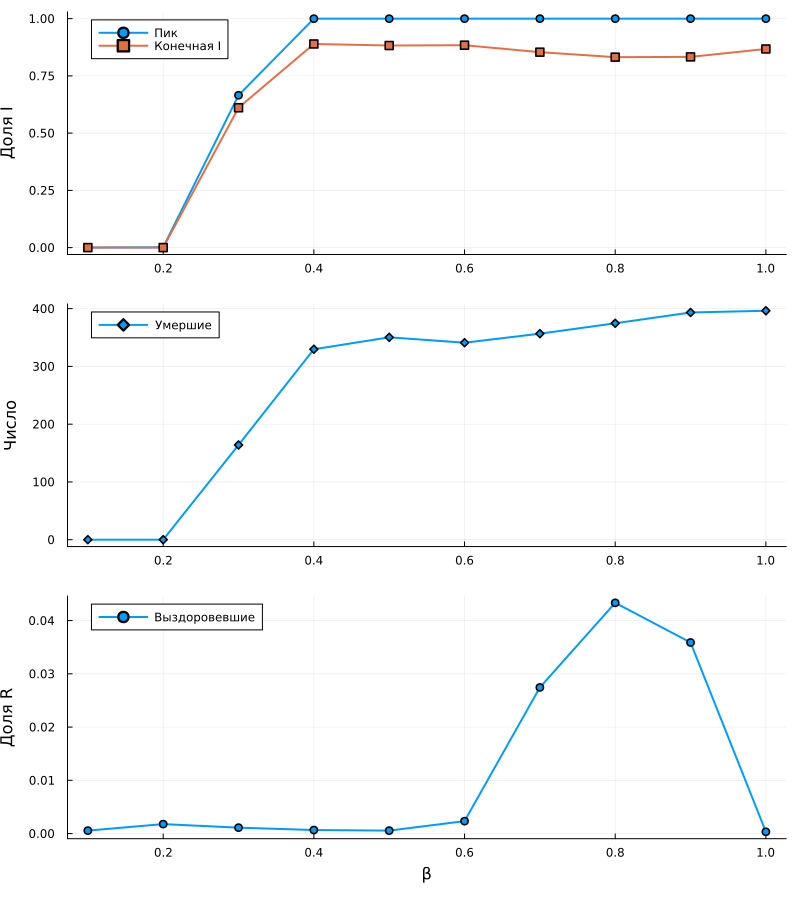
\includegraphics[width=0.85\linewidth,height=\textheight,keepaspectratio]{image/plots/comprehensive_analysis.png}
\end{column}
\end{columns}
\end{frame}

\begin{frame}{Литературное программирование}
\protect\phantomsection\label{ux43bux438ux442ux435ux440ux430ux442ux443ux440ux43dux43eux435-ux43fux440ux43eux433ux440ux430ux43cux43cux438ux440ux43eux432ux430ux43dux438ux435}
\begin{columns}[c]
\begin{column}{0.38\linewidth}
Все основные эксперименты оформлены в литературном стиле.

Из одного исходника автоматически создаются:

\begin{itemize}
\tightlist
\item
  Julia-скрипт;
\item
  Quarto-документ;
\item
  Jupyter Notebook.
\end{itemize}
\end{column}

\begin{column}{0.62\linewidth}
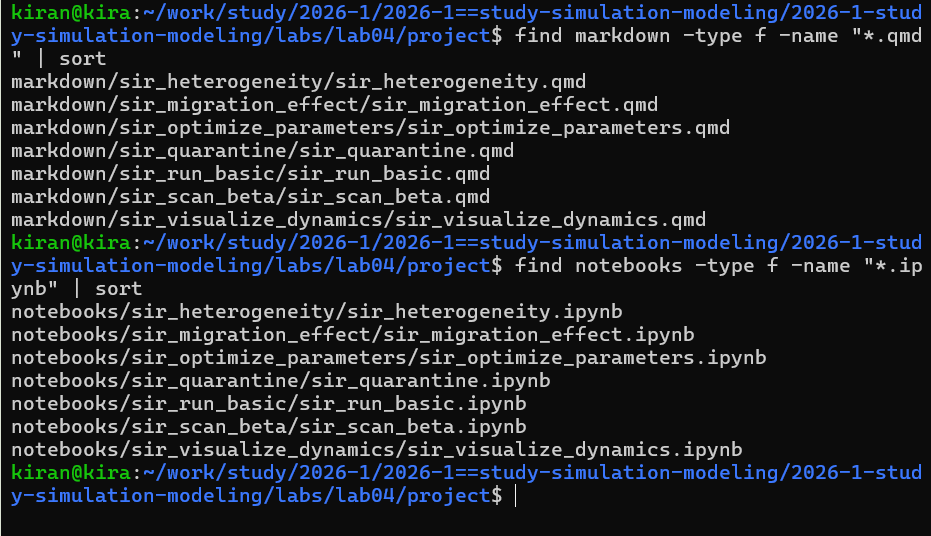
\includegraphics[width=1\linewidth,height=\textheight,keepaspectratio]{image/11.png}
\end{column}
\end{columns}
\end{frame}

\begin{frame}{Проверка воспроизводимости}
\protect\phantomsection\label{ux43fux440ux43eux432ux435ux440ux43aux430-ux432ux43eux441ux43fux440ux43eux438ux437ux432ux43eux434ux438ux43cux43eux441ux442ux438}
\begin{columns}[c]
\begin{column}{0.37\linewidth}
Все созданные Jupyter Notebook были повторно выполнены.

Таким образом проверяется, что эксперимент воспроизводится из
автоматически созданных файлов.
\end{column}

\begin{column}{0.63\linewidth}
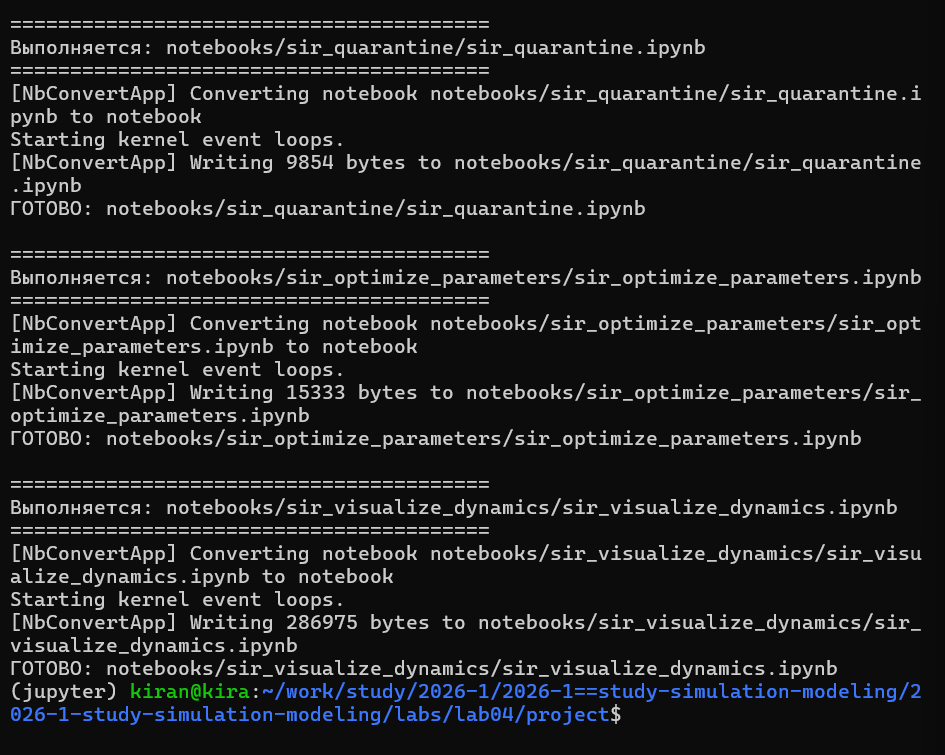
\includegraphics[width=1\linewidth,height=\textheight,keepaspectratio]{image/12.png}
\end{column}
\end{columns}
\end{frame}

\begin{frame}{Результаты разработки}
\protect\phantomsection\label{ux440ux435ux437ux443ux43bux44cux442ux430ux442ux44b-ux440ux430ux437ux440ux430ux431ux43eux442ux43aux438}
\begin{columns}[c]
\begin{column}{0.4\linewidth}
В проекте сохранены:

\begin{itemize}
\tightlist
\item
  ядро SIR-модели;
\item
  программы экспериментов;
\item
  CSV и JLD2 с результатами;
\item
  оригинальные PNG;
\item
  Quarto-документация;
\item
  Jupyter Notebook.
\end{itemize}
\end{column}

\begin{column}{0.6\linewidth}
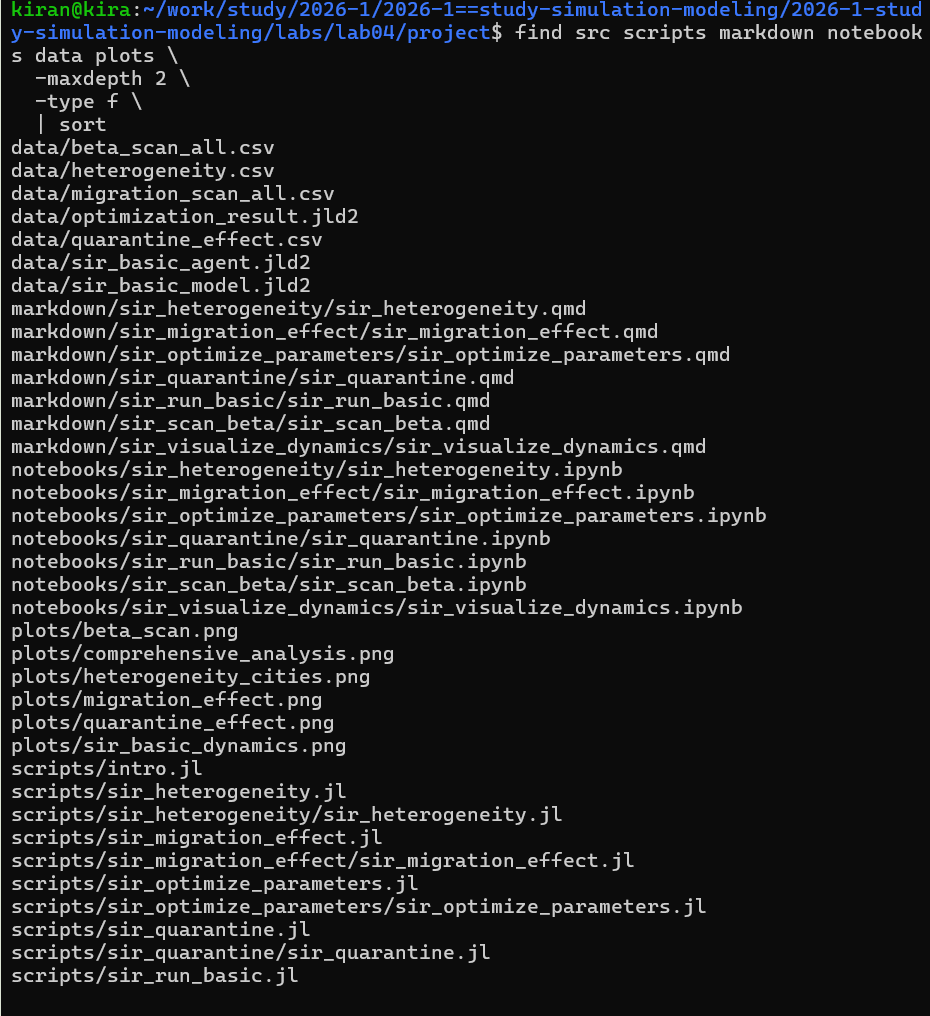
\includegraphics[width=1\linewidth,height=\textheight,keepaspectratio]{image/13.png}
\end{column}
\end{columns}
\end{frame}

\begin{frame}{Выводы}
\protect\phantomsection\label{ux432ux44bux432ux43eux434ux44b}
В лабораторной работе модель SIR реализована на уровне отдельных
агентов.

\begin{itemize}
\tightlist
\item
  исследован базовый эпидемический сценарий;
\item
  найден порог по коэффициенту заразности;
\item
  учтена неоднородность городов;
\item
  исследовано влияние миграции;
\item
  реализована карантинная мера;
\item
  выполнена оптимизация параметров.
\end{itemize}

\textbf{Все вычислительные эксперименты оформлены как воспроизводимый
Julia-проект.}
\end{frame}




\end{document}
